Los procesos se pueden simular con precisión LO para cualquier Lagrangian definida por el usuario, y la precisión NLO en el caso de correcciones QCD a procesos SM. También se pueden obtener elementos matriciales a nivel de árbol y un bucle.

necesitamos los siguientes programas:
\begin{itemize_f}
	\item  Generador de eventos - MadGraph (como generador de Monte Carlos) y Pythia ( como hadronizador ).
	\item  Simulador del detector - Delphes (con CMS card adecuado).
	\item  Análisis - C++ y Python.
\end{itemize_f}

La descripción general de todo el proceso se muestra en el diagrama \ref{fig:diagrama_workflow}, como se puede ver el generador de Monte Carlo utilizado para la generación de eventos es MadGraph5a\_MC. Es un marco que tiene como objetivo proporcionar todos los elementos necesarios para la fenomenología SM y la inclusión del Susy, como los cálculos de secciones transversales, la generación de eventos difíciles y su coincidencia con generadores de eventos, y el uso de una variedad de herramientas relevantes para la manipulación de eventos y análisis. Los procesos se pueden simular con precisión para cualquier Lagrangiano definido por el usuario. MadGraph toma entradas en forma de varios string mostrados a continuación:
\begin{itemize_f}
	\item  proc\_card.dat - descripción del proceso.
	\item  param\_card.dat - masa, decaimiento y otros parámetros del modelo.
	\item  run\_card.dat - energía del emisor, pdfset and otras configuraciones de colisión.
\end{itemize_f}

\begin{figure}[h!]
    \centering
    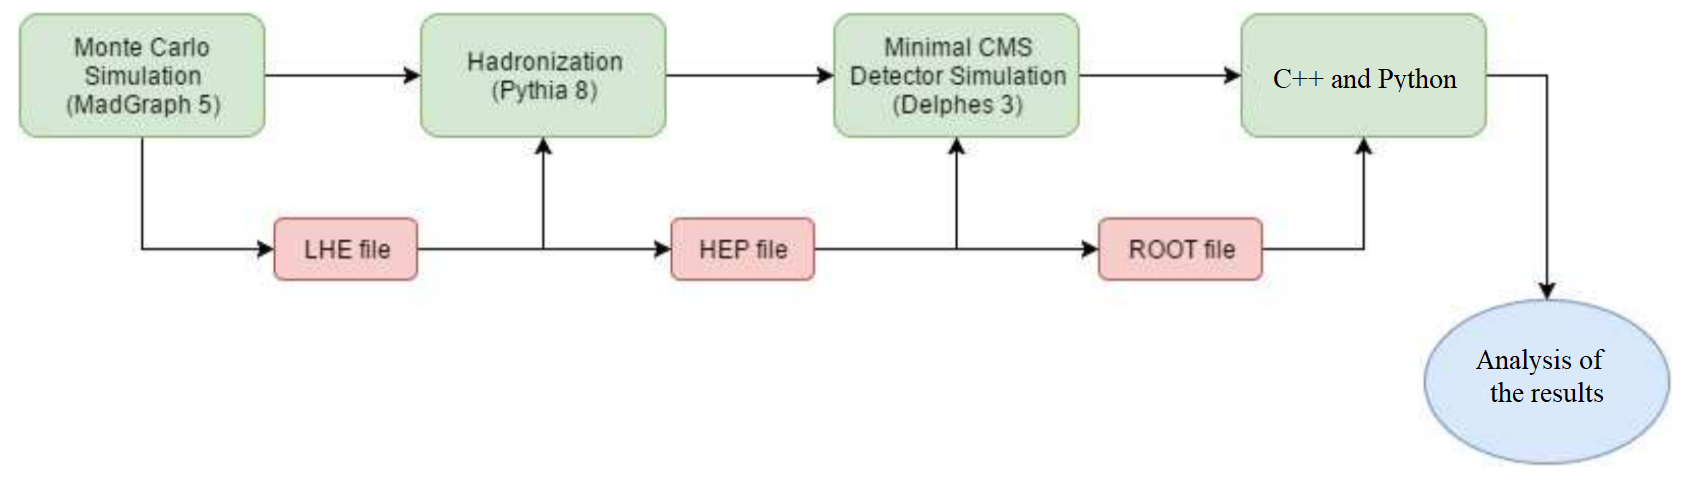
\includegraphics[width=0.84\textwidth]{Analisis_y_Resultados/imagenes/diagrama_workflow.png}
    \caption{Diagrama de flujo de la investigación.}
    \label{fig:diagrama_workflow}
\end{figure}

